\documentclass[a4paper, 12pt]{article}
\usepackage[utf8]{inputenc}
\usepackage[T2A]{fontenc}
\usepackage{tablefootnote}
\usepackage{footnote}
\usepackage{indentfirst}
\usepackage{amsmath}
\usepackage{graphicx}
\usepackage{wrapfig}
\usepackage{color}
\usepackage{subcaption}
\usepackage[export]{adjustbox}
\usepackage{float}
\usepackage{cite}
\usepackage{caption}
\usepackage{textcomp}
\usepackage{color,colortbl}
\definecolor{col0}{RGB}{147, 30, 206}
\definecolor{col1}{RGB}{136, 117, 98}
\definecolor{col2}{RGB}{152, 127, 113}
\definecolor{col3}{RGB}{152, 127, 110}
\definecolor{col4}{RGB}{145, 122, 103}
\definecolor{col5}{RGB}{140, 119, 102}
\definecolor{col6}{RGB}{143, 121, 103}
\definecolor{col7}{RGB}{164,109,89}
\definecolor{col8}{RGB}{141, 120, 103}
\definecolor{col9}{RGB}{144, 121, 103}
\definecolor{col10}{RGB}{145,123, 105}




\title{DSBA SUMMER PRACTICE TASK}
\author{Vadim Khanin}
\date{July 2022}
\begin{document}
\maketitle
\newpage
\begin{center}
\tableofcontents
\end{center}
\newpage


    
\section{Abstract}

The purpose of this document is to learn basic ideas about working with LaTeX\cite{lamport1985i1}.


\section{Introduction}
Since my coursework report hardly has any formulas or tables ,the following document will also include tables, formulas and images from other sources.
\newpage
\begin{center}
\large
\section{Tables} 

\subsection{First Table}
\begin{savenotes}
\begin{table}[H]
    \centering
    \begin{tabular}{| c | c | c | c | c |}
\hline
 \multicolumn{5}{|c|}{ANOVA\footnote{ANalysis Of VAriance} table} \\
 \hline
  Source & DF\footnote{degrees of freedom} & SS & MS & F-score \\
  \hline
  row & 2 & 293.19 & 420. & -7.04 \\ 
  column & 2 & 161.19 & 406 & -3.9 \\ 
  errors & 4 & 83.19 & - & - \\
  Total & 8 & 371.191 & 429.33 & - \\ 
  \hline
\end{tabular}
    \caption{ANOVA table with arbitary numbers}
    \label{tab:l1}
\end{table}


\subsection{Second Table}
\begin{table}[H]
    \centering
    \begin{tabular}{|c|c|c|c|}
\hline \rowcolor{col0}
& \multicolumn{3}{c|}{RGB-values} \\
\cline{2-4} \rowcolor{col0}
\raisebox{1.5ex}[0cm][0cm]{\textnumero of color bar}
& Red & Green & Blue \\ \rowcolor{col1}
\hline
1 &  136  &   117  &   98  \\ \rowcolor{col2}
\hline
2 &  152  &   127  &   113 \\ \rowcolor{col3}
\hline
3 &  152  &   127  &   110 \\ \rowcolor{col4}
\hline
4 &  145  &   122  &   103 \\ \rowcolor{col5}
\hline
5 &  140  &   119  &   102 \\ \rowcolor{col6}
\hline
6 &  143  &   121  &   103 \\ \rowcolor{col7}
\hline
7 &  164  &   109  &   89  \\ \rowcolor{col8}
\hline
8 &  141  &   120  &   103 \\ \rowcolor{col9}
\hline
9 &  144  &   121  &   103 \\ \rowcolor{col10}
\hline
10 &  145 &   123  &   105   \\
\hline
\end{tabular}
    \caption{Some complex table based on data from my coursework.The lines are colored in the color of its rgb values.}
    \label{tab:l2}
\end{table}
\end{savenotes}
\end{center}


\newpage



\section{Formulas}

\subsection{formula 1}
The following formula is taken from my coursework.


Let $V_k = (R_i,G_i,B_i)$ be the rgb values of i-th color bar of the k-th volunteer and $U_k = (R_i,G_i,B_i)$ be the rgb values of the j-th  color bar of the k-th volunteer. Then: 
$$\forall i,j\in [1;2) \cup (2;10]$$ such that $$i \neq j$$
\begin{equation*}
 \begin{cases}
  |R_i-R_j|\leq5 \\
  |G_i-G_j|\leq4 \\
  |B_i-B_j|\leq5
 \end{cases}
\end{equation*}
\begin{equation*}
 \begin{cases}
  R^*=0.97 \\
  R^*=0.97 \\
  R^*=0.97
 \end{cases}
\end{equation*}

\subsection{formula 2} %По каким-то причинам Латеху не нравятся переносы формул
Some task from first course calculus hw redone in LaTeX.
\newline
\newline
\large
$$\int_{-1}^{3} \frac{dx}{\sqrt{x^2+4x+3}}=\int_{-1+\epsilon}^{3} \frac{dx}{\sqrt{(x+2)^2-1}}=$$\\
$$=\lim_{\epsilon\to 0}(\ln{|\sqrt{(x+2)^2-1}+x+2|)\bigg|_{-1+\epsilon}^{3}}=$$\\
$$=\lim_{\epsilon\to 0}(\ln{|\sqrt{24}+5|}-\ln{\sqrt{(1+\epsilon)^2}-1+\epsilon+2})=$$\\
$$=\ln{|\sqrt{24}+5|}\approx 2.3$$
\normalsize
\subsection{formula 3}
Some random formula.
\LARGE
$$\omega(x,t,n)=\sqrt{\frac{\lim_{x\to 0} (1+x^{-2})^{x^2}}{\int_{0}^{x}\frac{sin t}{1+cos^2 t}\,dt}}\cdot\sum_{n=1}^n\frac{1}{n^2}$$
\normalsize 
\subsection{formula 4}
Some task from this year calculus redone in LaTeX.
\large
$$S_1 = \iint_{D}r\,dr\,d\phi=\int_{0}^{\frac{\pi}{3}}\,d\phi\int_{0}^{sin 3\phi}r\,dr=\int_{0}^{\frac{\pi}{3}}(\frac{r^2}{2}\bigg|_{0}^{sin3\phi})\,d\phi=\int_{0}^{\frac{\pi}{3}} \frac{sin^2 3\phi}{2}\,d\phi=$$\\
$$=\int_{0}^{\frac{\pi}{3}} \frac{1-cos6\phi}{4}\,d\phi=(\frac{1}{4}\phi-\frac{sin6\phi}{24})\bigg|_{0}^{\frac{\pi}{3}}=\frac{\pi}{12}-\frac{sin2\pi}{12}=\frac{\pi}{12}$$
\normalsize
\newpage

\section{Lists}
Example of making a large nested list with ordered and unordered sublists.
\begin{enumerate}
    \item First item
    \begin{itemize}
    \item cdot item
    \item[$\chi$] $\chi-item$
        \begin{enumerate}
            \item item a
            \begin{itemize}
                \item[$\longrightarrow$] Some Item with arrow
                \item[$\kappa$] kappa item
            \end{itemize}
            \item item b
        \end{enumerate}
    \end{itemize}
    \item Second item
    \begin{enumerate}
        \item another a item 
        \item another b item 
        \item item c
        \begin{enumerate}
            \item item i 
            \item item ii
            \item item iii
            \begin{enumerate}
                \item item A
                \item item B
                \begin{itemize}
                    \item sub B item
                    \item another sub B item 
                \end{itemize}
            \end{enumerate}
        \end{enumerate}
    \end{enumerate}
    \item Third item
    \begin{itemize}
        \item[$	\bar{A}$] A bar item
        \item [$\dot{\sigma}$] sigma-dot item 
        \begin{itemize}
            \item another sub item 
            \begin{itemize}
                \item another subsubitem
            \end{itemize}
            \item another sub item 
        \end{itemize}
    \end{itemize}
\end{enumerate}
\newpage


\section{Images}
Examples of working with images.

\begin{figure}[h]
    \centering
    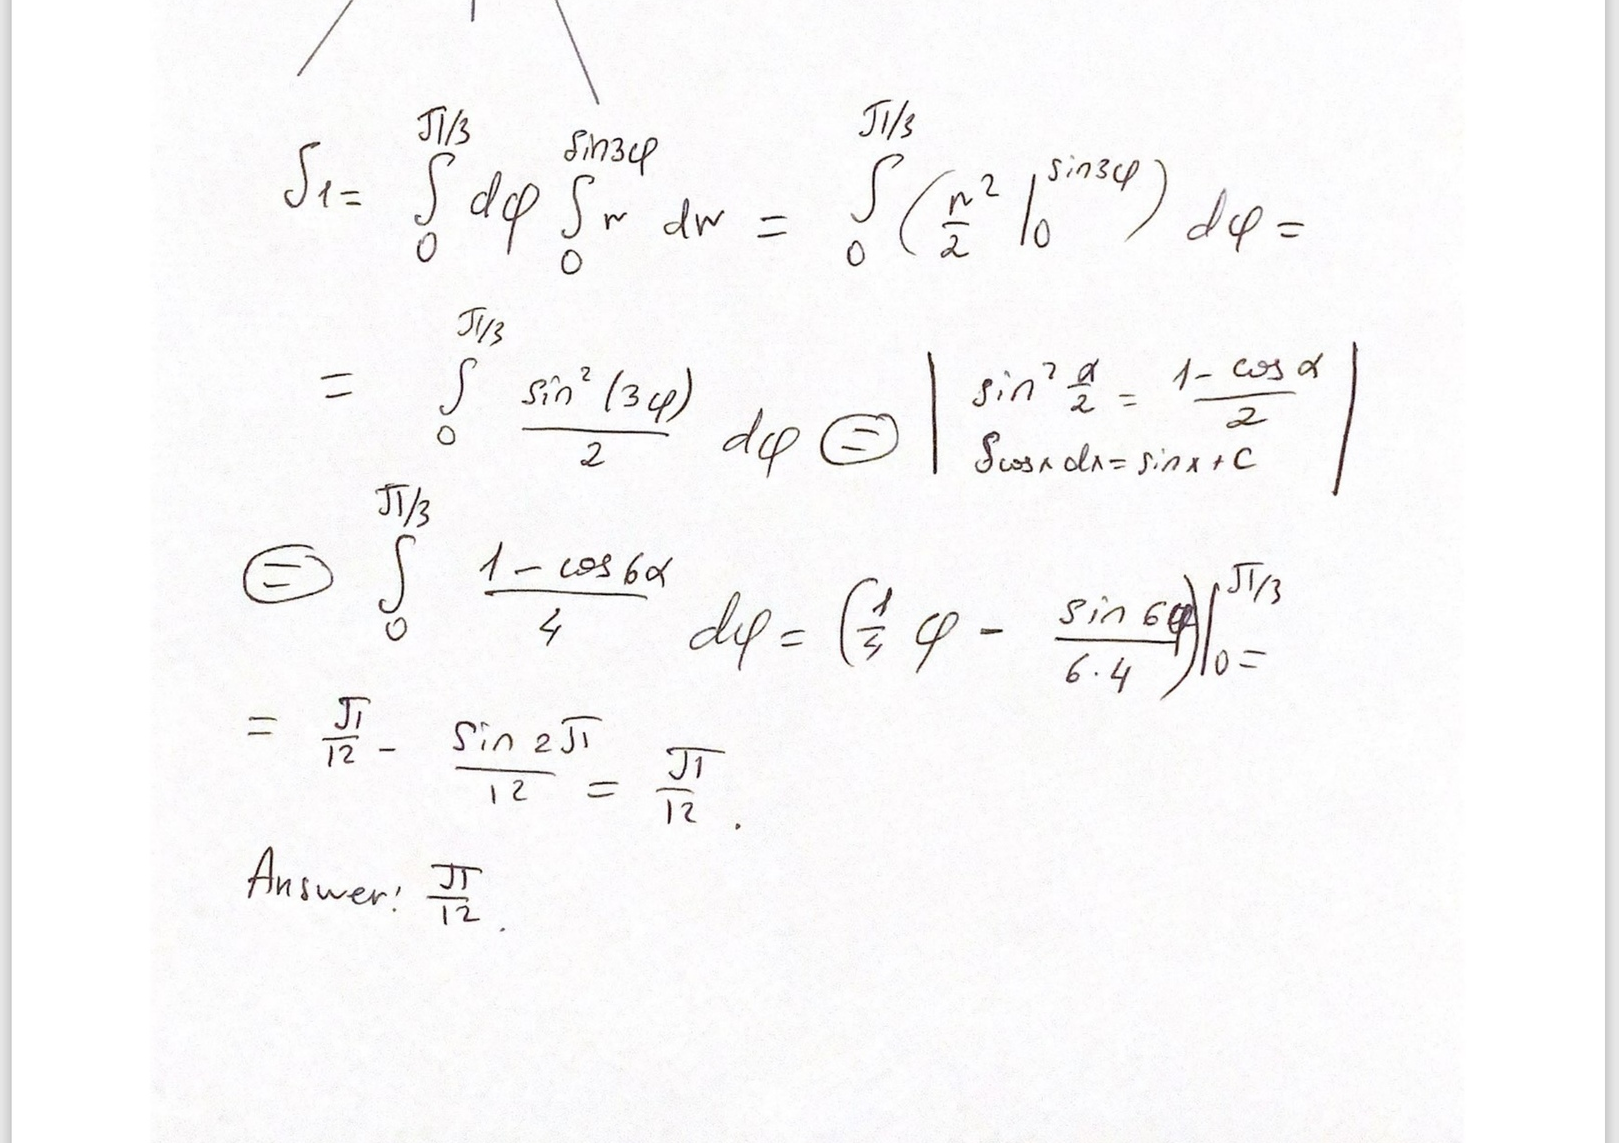
\includegraphics[width=1\linewidth, right]{im1.png}
    \caption{formula 4}
    \label{fig1}
\end{figure}
\begin{wrapfigure}{l}{0.4\textwidth}
    \centering
    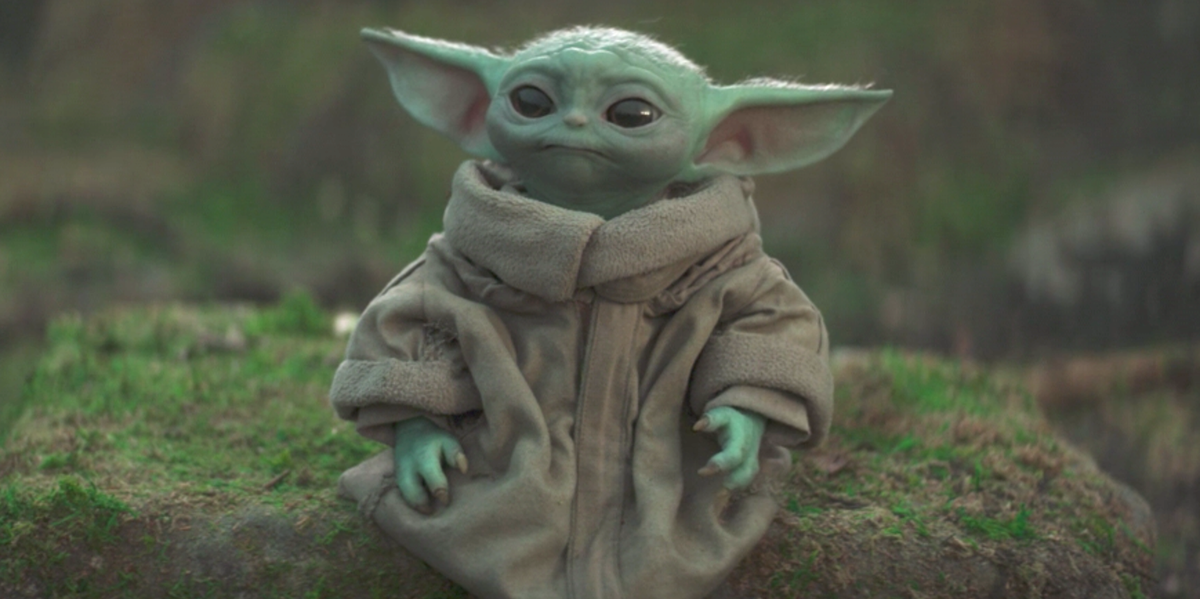
\includegraphics[width=0.4\textwidth]{im2.png}
    \caption{Grogu}
\end{wrapfigure}
You may notice, that formula on figure \ref{fig1} is formula, which was LaTeXed before.You may also notice that there is baby yoda\cite{rocha2022baby} to the left\footnote[1]{showing that I know how to place the image there} from this text. Bellow, on figure \ref{fig2} there are color bars from my coursework(linked together using LaTeX). Each color bar represent changes in dominant color of the image. As you may see in general, the changes are hardly visible by eyes.
\begin{figure}[H]
    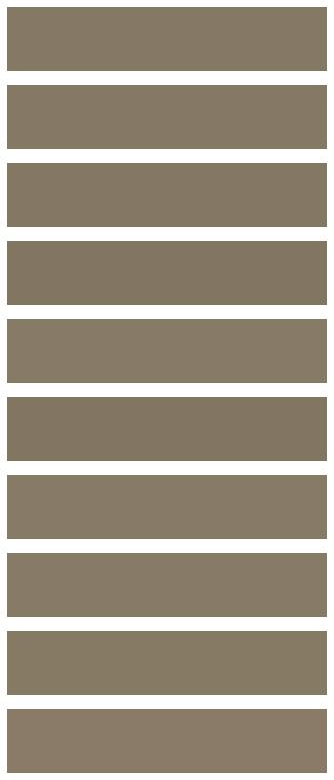
\includegraphics[width=.1\linewidth]{vid1_bar.jpg}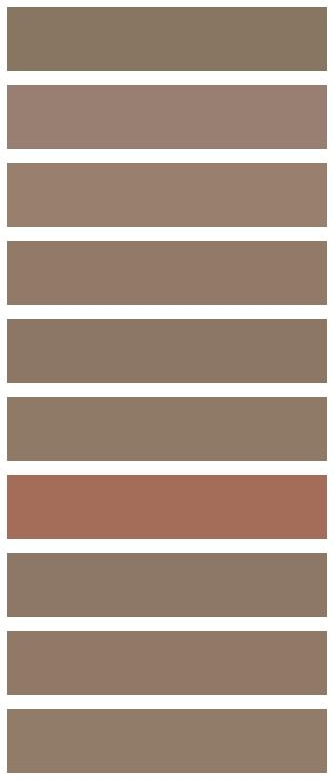
\includegraphics[width=.1\linewidth]{vid2_bar.jpg}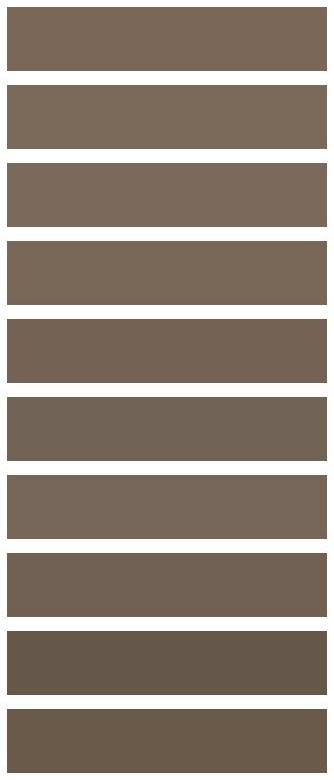
\includegraphics[width=.1\linewidth]{vid3_bar.jpg}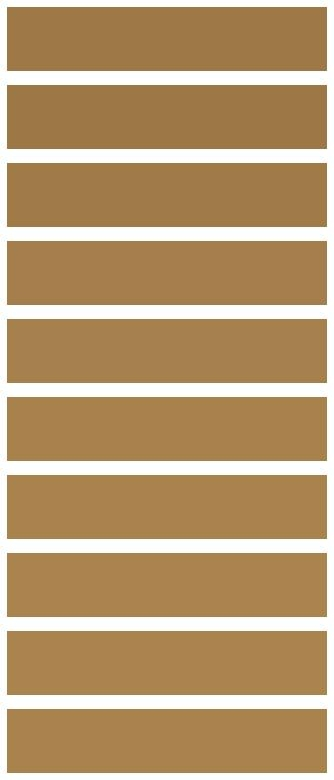
\includegraphics[width=.1\linewidth]{vid4_bar.jpg}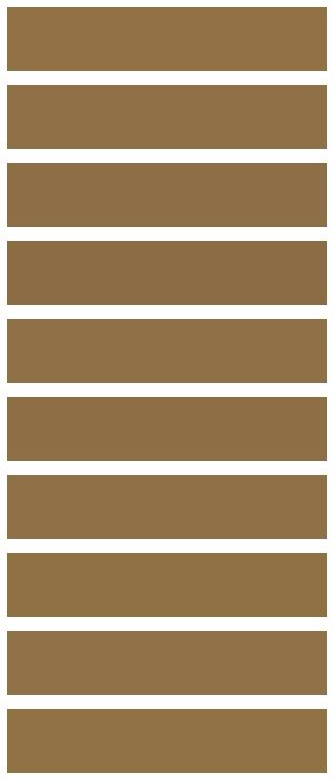
\includegraphics[width=.1\linewidth]{vid5_bar.jpg}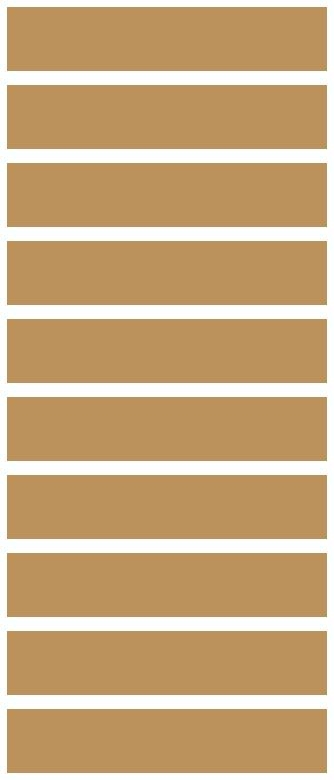
\includegraphics[width=.1\linewidth]{vid6_bar.jpg}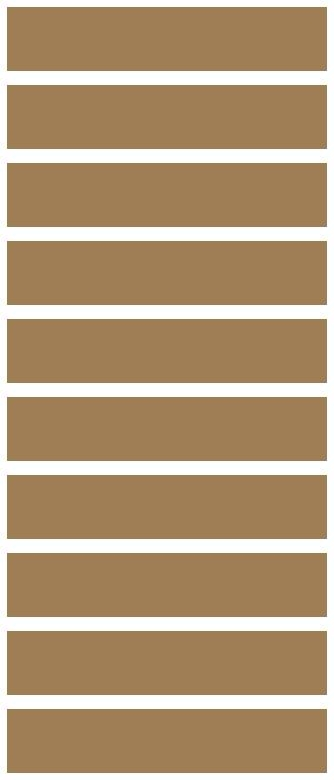
\includegraphics[width=.1\linewidth]{vid7_bar.jpg}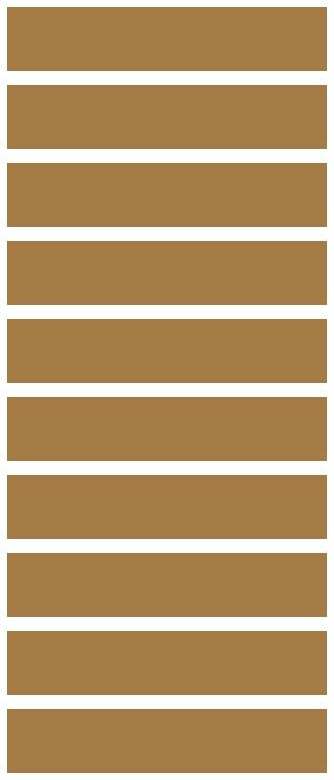
\includegraphics[width=.1\linewidth]{vid8_bar.jpg}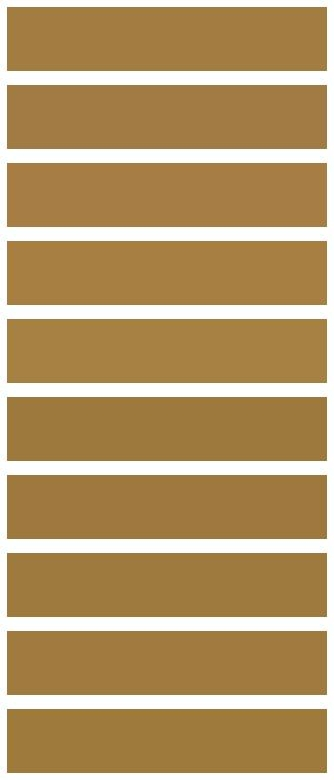
\includegraphics[width=.1\linewidth]{vid9_bar.jpg}
    \caption{}
    \label{fig2}
\end{figure}

\begin{wrapfigure}{r}{0.25\textwidth} %this figure will be at the right
    \centering
    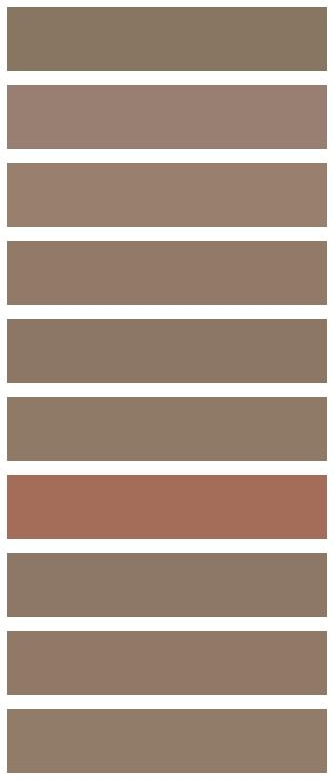
\includegraphics[width=0.1\textwidth]{vid2_bar.jpg}
    \caption{}
    \label{fig3}
\end{wrapfigure}
However for the second bar, they can be clearly seen. This bar is now to the right from this text on figure \ref{fig3}. The rgb values of this bar a represented in table \ref{tab:l2} on page \pageref{tab:l2}. Below, there are some images rotated and scaled using LaTeX.
\newline

\includegraphics[scale=0.24,angle=15]{im3.jpg}
\newline

\includegraphics[scale=0.12,angle=30]{im3.jpg}
\newline

\includegraphics[scale=0.06,angle=45]{im3.jpg}
\newline

\includegraphics[scale=0.03,angle=60]{im3.jpg}
\newline

\includegraphics[scale=0.06,angle=90]{im3.jpg}
\newline

\includegraphics[scale=0.12,angle=105]{im3.jpg}

\includegraphics[scale=0.12,angle=120]{im3.jpg}

\includegraphics[scale=0.12,angle=150]{im3.jpg}

\includegraphics[scale=0.12,angle=165]{im3.jpg}
\begin{flushright}
The end. 
\end{flushright}


\bibliographystyle{abbrv}
\bibliography{bib.bib}
\end{document}


